\chapter{Experiments}
\label{chap:experiments}

Multiple experiments are conducted in this paper. They test the performance of different scattering architectures, i.e. sequential and parallel, and compare them to the standard architecture on different datasets. \\
Section \ref{sec:datasets} gives a general overview of the datasets used in this paper. Section \ref{sec:setup} shows what kind of setup was used for the architectures to conduct the experiments. The reproduction experiments of the classification results on different datasets is set up in Section \ref{sec:classification_experiments} where the main experiments for object detection are described in Section \ref{sec:object_detection_experiments}.

	
\section{Datasets}
\label{sec:datasets}

The experiments in this work were conducted on multiple datasets. Two of them are known and openly available datasets for benchmarking purposes, namely PASCAL VOC and KITTI. The other five datasets used were specifically created for this work to test the geometric properties of the scattering transform for object detection tasks. 

\subsection{PASCAL VOC}

The PASCAL Visual Object Classes dataset is a common benchmark for object detection tasks \cite{VOC}. This work uses a combination of VOC images from 2007 and 2012 totaling 27088 images. They are split in test and training set such that the training set contains around 16k images. There are 20 different classes in the dataset that are frequently seen in a person's daily life ranging from aeroplane over bicycle to TV monitor. Most images are taken such that the object is centered and only one object is seen. In some rare instances two or more objects are seen in the same image, i.e. when a person is riding a horse or two cats are playing together. To get a feeling for the dataset Figure \ref{fig:VOC_samples} shows three sample images from PASCAL VOC.

\begin{figure}[!htb]
	\centering
	\begin{tabular}{ccc}
		\subfloat[]{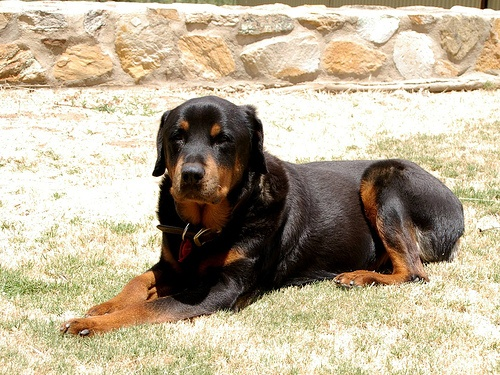
\includegraphics[width=3cm]{images/VOC_sample_1.jpg}} 
		& \subfloat[]{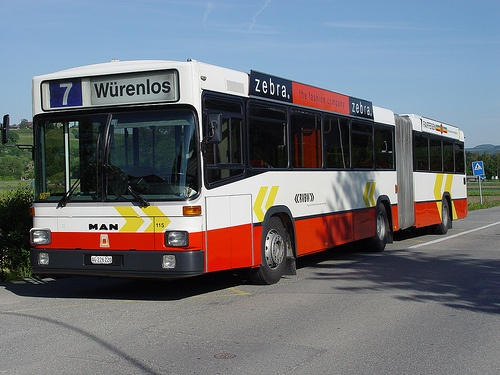
\includegraphics[width=3cm]{images/VOC_sample_2.jpg}}&
		\subfloat[]{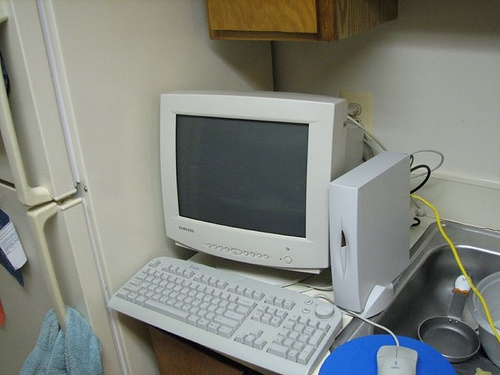
\includegraphics[width=3cm]{images/VOC_sample_3.jpg}}
	\end{tabular}
	\caption{Three samples from the PASCAL VOC dataset showing a dog, bus and TV monitor from left to right.}
	\label{fig:VOC_samples}
\end{figure}

\subsection{KITTI}

The KITTI Vision dataset is specifically created for object detection of traffic scenes \cite{Geiger2013IJRR}. It has four classes: cars, cyclists, pedestrians and miscellaneous. The entire dataset has around 8k images and is split in around 6k training and 2k test images for this work. The scenes visible in the KITTI dataset contain multiple objects, i.e. multiple cars, cyclists and pedestrians in the same image and are therefore significantly harder to detect compared to PASCAL VOC. The original images are taken with aspect ratio 3:1. The SSD setup used in this paper uses an input size of 300 by 300 thereby reshaping the image and most objects in it which could pose problems. A SSD with input size of 1000 by 300 was setup but did not yield better results (see \ref{sec:stuff_that_did_not_work} for the description of a negative result). Four traffic scenes are depicted in Figure \ref{fig:kitti_samples}. 

\begin{figure}[!htb]
	\centering
	\begin{tabular}{cc}
		\subfloat[]{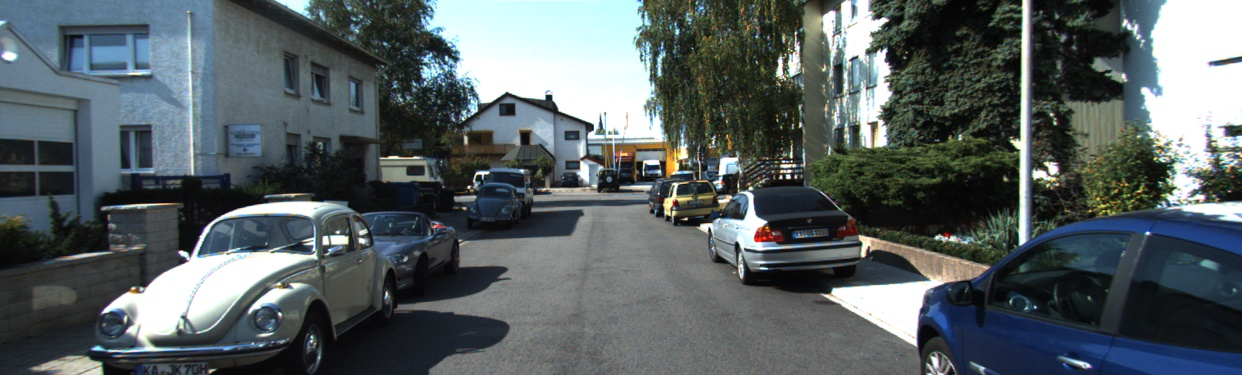
\includegraphics[width=7cm]{images/kitti_sample_1.jpg}} 
		& \subfloat[]{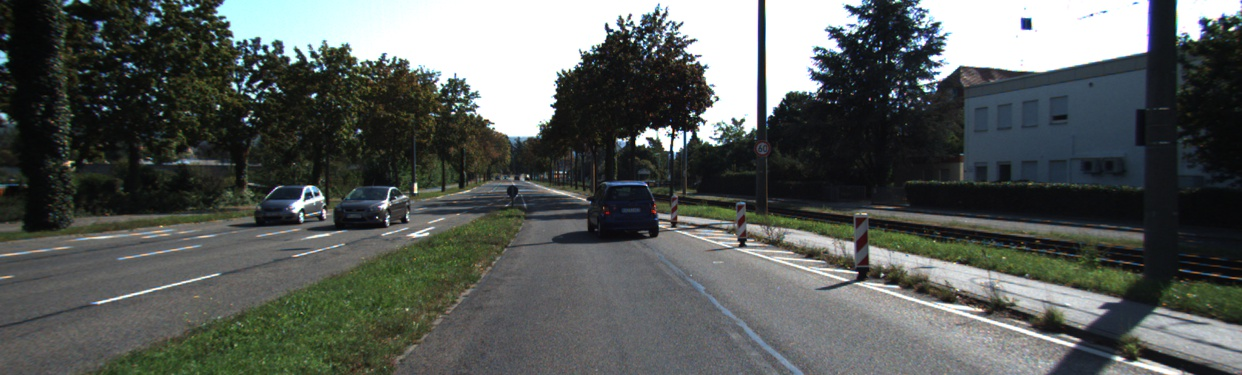
\includegraphics[width=7cm]{images/kitti_sample_2.jpg}} \\
		\subfloat[]{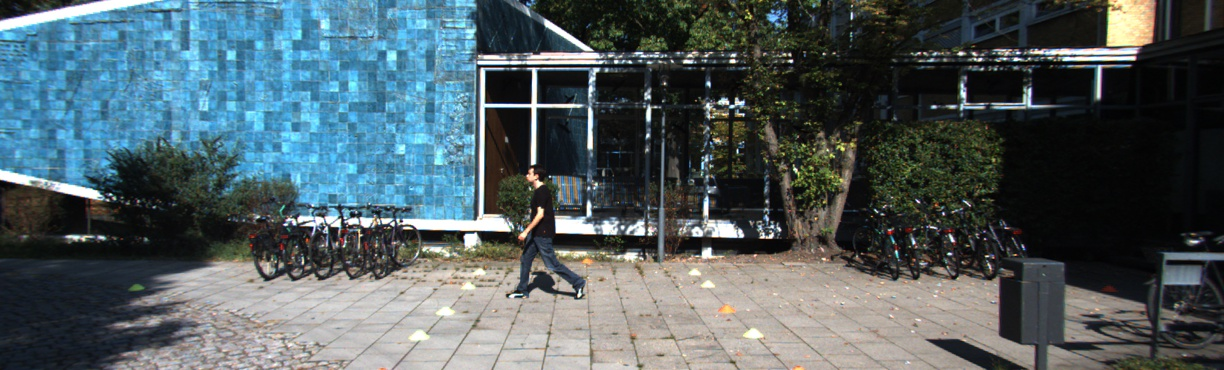
\includegraphics[width=7cm]{images/kitti_sample_3.jpg}} 
		& \subfloat[]{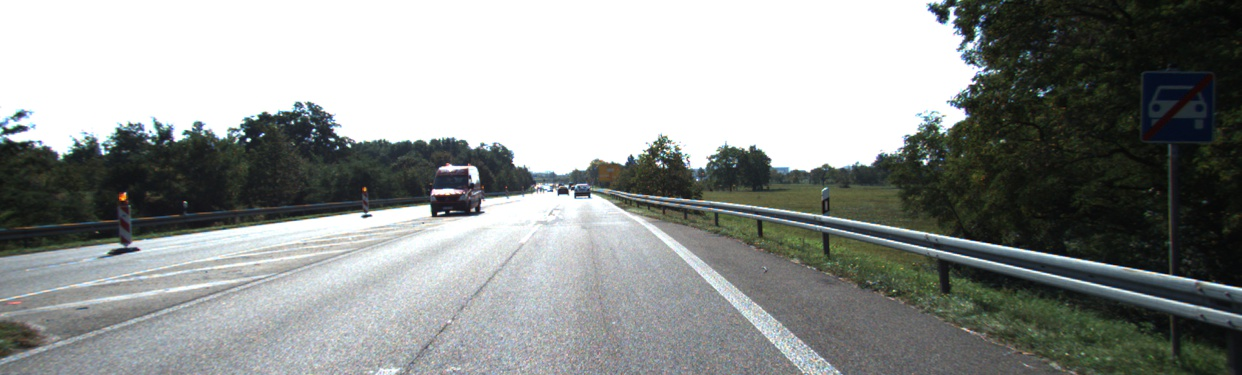
\includegraphics[width=7cm]{images/kitti_sample_4.jpg}} 
	\end{tabular}
	\caption{Four samples from the KITTI dataset.}
	\label{fig:kitti_samples}	
\end{figure}

\subsection{Toy Data}

To test the quality of the networks on easier datasets with simple geometric properties a toy data set was constructed. Every image contains three objects that can also be overlayed. Every object has one of three randomly chosen colors. The objects are either a triangle, a rectangle or an ellipse. In total 6k such images are contained in the training set and 2k in the test set. Four samples can be found in Figure \ref{fig:toy_data_samples}

\begin{figure}[!htb]
	\centering
	\begin{tabular}{cccc}
		\subfloat[]{\fbox{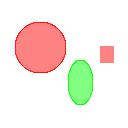
\includegraphics[width=2.8cm]{images/toy_data/0010001.jpg}}} 
		& \subfloat[]{\fbox{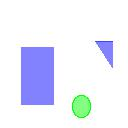
\includegraphics[width=2.8cm]{images/toy_data/0010002.jpg}}} &
		\subfloat[]{\fbox{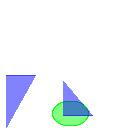
\includegraphics[width=2.8cm]{images/toy_data/0010005.jpg}}}  &
		\subfloat[]{\fbox{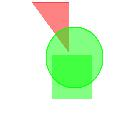
\includegraphics[width=2.8cm]{images/toy_data/0010006.jpg}}} 
	\end{tabular}
	\caption{Four samples from the toy data set.}
	\label{fig:toy_data_samples}
\end{figure}

\subsection{Test Invariances Toy Data}

To test the invariances individually four additional datasets have been created. All of them contain only one object per image. They are all created in the same procedure: A base image with a randomly chosen object is created and put in the training set. Six further images are derived from the base image w.r.t. the particular invariance and put into the test set. This is done 1000 times per dataset resulting in 1k training and 6k test images per invariance. All objects have one of three randomly chosen colors such that the network does not learn to predict based on the color. The specific procedures are described in the following and samples are provided.

\subsubsection{Scale}

A base image is created as explained above. Six further images are created by scaling the object with factors from 0.5 to 1.5 of the original size. The objects are triangles, rectangles and ellipses. Samples can be seen in Figure \ref{fig:scale_samples}.

\begin{figure}[!htb]
	\centering
	\begin{tabular}{cccc}
		\subfloat[]{\fbox{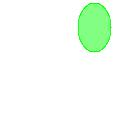
\includegraphics[width=2.8cm]{images/scale_data/0000000_00.jpg}}} 
		& \subfloat[]{\fbox{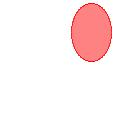
\includegraphics[width=2.8cm]{images/scale_data/0000000_03.jpg}}} &
		\subfloat[]{\fbox{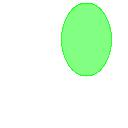
\includegraphics[width=2.8cm]{images/scale_data/0000000_09.jpg}}}  &
		\subfloat[]{\fbox{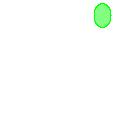
\includegraphics[width=2.8cm]{images/scale_data/0000000_10.jpg}}} 
	\end{tabular}
	\caption{Four samples from the scale toy data set. a) is the base image; b) -d) are the scaled versions}
	\label{fig:scale_samples}
\end{figure}

\subsubsection{Rotation}

A base image is created as explained above. Ten further images are created by rotating the object around its own center with equal angle sizes. The objects are triangles, rectangles and heptagons. Samples can be seen in Figure \ref{fig:rotation_samples}.

\begin{figure}[!htb]
	\centering
	\begin{tabular}{cccc}
		\subfloat[]{\fbox{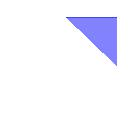
\includegraphics[width=2.8cm]{images/rotation_data/0000000_00.jpg}}} 
		& \subfloat[]{\fbox{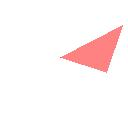
\includegraphics[width=2.8cm]{images/rotation_data/0000000_03.jpg}}} &
		\subfloat[]{\fbox{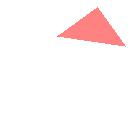
\includegraphics[width=2.8cm]{images/rotation_data/0000000_09.jpg}}}  &
		\subfloat[]{\fbox{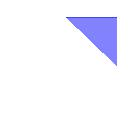
\includegraphics[width=2.8cm]{images/rotation_data/0000000_10.jpg}}} 
	\end{tabular}
	\caption{Four samples from the rotation toy data set. a) is the base image; b) -d) are the rotated versions}
	\label{fig:rotation_samples}
\end{figure}

\subsubsection{Deformation}

A base image is created as explained above. Ten further images are created by taking one point of the object and adding noise to it. The noise is uniformly distributed and capped such that it can maximally add or subtract 20\% of the original object size to the point.  The objects are triangles, rectangles and heptagons. Samples can be seen in Figure \ref{fig:deformation_samples}.

\begin{figure}[!htb]
	\centering
	\begin{tabular}{cccc}
		\subfloat[]{\fbox{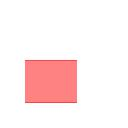
\includegraphics[width=2.8cm]{images/deformation_data/0000001_00.jpg}}} 
		& \subfloat[]{\fbox{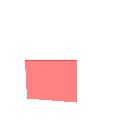
\includegraphics[width=2.8cm]{images/deformation_data/0000001_03.jpg}}} &
		\subfloat[]{\fbox{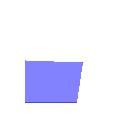
\includegraphics[width=2.8cm]{images/deformation_data/0000001_09.jpg}}}  &
		\subfloat[]{\fbox{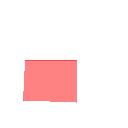
\includegraphics[width=2.8cm]{images/deformation_data/0000001_10.jpg}}} 
	\end{tabular}
	\caption{Four samples from the deformation toy data set. a) is the base image; b) -d) are the deformed versions}
	\label{fig:deformation_samples}
\end{figure}

\subsubsection{Translation}

A base image is created as explained above. Ten further images are created by changing the location in the image randomly. The objects are triangles, rectangles and ellipses. Samples can be seen in Figure \ref{fig:translation_samples}.

\begin{figure}[!htb]
	\centering
	\begin{tabular}{cccc}
		\subfloat[]{\fbox{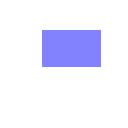
\includegraphics[width=2.8cm]{images/translation_data/0000017_00.jpg}}} 
		& \subfloat[]{\fbox{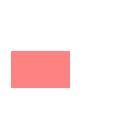
\includegraphics[width=2.8cm]{images/translation_data/0000017_03.jpg}}} &
		\subfloat[]{\fbox{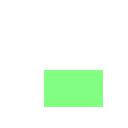
\includegraphics[width=2.8cm]{images/translation_data/0000017_09.jpg}}}  &
		\subfloat[]{\fbox{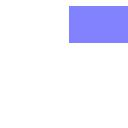
\includegraphics[width=2.8cm]{images/translation_data/0000017_10.jpg}}} 
	\end{tabular}
	\caption{Four samples from the translation toy data set. a) is the base image; b) -d) are the translated versions}
	\label{fig:translation_samples}
\end{figure}

\subsection{Classification Toy Data}

To reproduce the results of \cite{ScalingTheScatteringTransform2017} regarding classification a network is trained on a toy dataset created for classification. Every image contains exactly one triangle, ellipse or rectangle in different sizes and colors.The data from the object detection toy data cannot be reused because they contain three objects per image instead of just one. Samples of the images are shown in Figure \ref{fig:toy_data_class_samples}.

\begin{figure}[!htb]
	\centering
	\begin{tabular}{cccc}
		\subfloat[]{\fbox{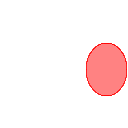
\includegraphics[width=2.8cm]{images/toy_data_classification/sample_1.png}}} 
		& \subfloat[]{\fbox{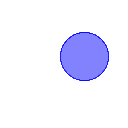
\includegraphics[width=2.8cm]{images/toy_data_classification/sample_2.png}}} &
		\subfloat[]{\fbox{
\includegraphics[width=2.8cm]{images/toy_data_classification/sample_4.png}}}  &
		\subfloat[]{\fbox{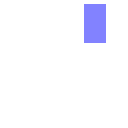
\includegraphics[width=2.8cm]{images/toy_data_classification/sample_7.png}}} 
	\end{tabular}
	\caption{Four samples from the classification toy data set.}
	\label{fig:toy_data_class_samples}
\end{figure}


\section{Setup}
\label{sec:setup}

In the following section technical specificities are explained to further understand and potentially reproduce the findings of this work. The code for the experiments has been implemented in Python3, and PyTorch \cite{Pytorch} was used as a framework for the neural networks. The code can also be accessed at \url{https://github.com/mariushobbhahn/CompSci_Bachelor_201819}.


\subsection{Augmentations, Batchnorm, Multibox Loss, Optimizer} 

Since neural networks have become so popular many pre-processing steps and techniques applied during the forward pass have become successful and standard. In this subsection is a description of the different approaches that were chosen for the experiments. In all cases the images are reshaped to fit the SSD setup to have a size of 300x300 pixels with three color channels. A data augmentation preprocessing step consists of photometric distortions, i.e. random contrast and saturation or changing the color representation of the image, random sample cropping and random mirroring of the data. The effectiveness of these augmentations is tested in the baseline experiments. \\
When the data has entered the network some other techniques can be applied during the forward pass. Using batch norm \cite{BatchNorm} is one popular tool. It consists of standardizing every batch to be distributed according to a Gaussian with mean 0 and standard deviation 1. This is done to speed up the training by preventing internal covariance shifts in the forward pass. The effectiveness of this technique is also tested in the baseline experiments. \\
To evaluate the quality of the proposals a metric is needed. The SSD works with the Multibox Loss. It is defined as 
\begin{equation}
	\label{eq:multibox_loss}
	L(x,c,l,g) = \frac{1}{N}(L_{\text{conf}} (x,c) + \alpha L_{\text{loc}} (x,l,g))
\end{equation}
where $x^p_{ij}=\{1,0\}$ is an indicator for matching the i-th default box to the j-th ground truth box of category $p$, $c$ are the class confidences, $l$ are the predicted box and $g$ the ground truth box parameters. Overall the multibox loss is a weighted sum of the localization loss $L_{\text{loc}}$ which is a smooth L1-loss between the predicted and ground truth box, and the confidence loss $L_{\text{conf}}$ which is a softmax loss over multiple classes. The technical details can be found in the original SSD paper \cite{SSD}. The multibox loss combines the regression task of finding the correct bounding boxes and classification task of finding the correct objects for those boxes. \\
The training objective is optimized using Stochastic Gradient Descent (SGD). Other optimizers such as Adam were tried but did not change the result in any way. 

\subsection{Hyperparameters}
\label{subsec:hyperparameters}

SSD has many hyperparameters over which can be optimized. A full list can be found in Table \ref{table:hyperparameters}.

\begin{table}[!htb]
	\centering
	\caption{Hyperparameters for the SSD. Explanations for some parameters are given in the accompanying text. The upper part of the list is concerned with the optimization, the lower part with the setup for the SSD.}
	\begin{tabularx}{\textwidth}{ X  X}
		\hline
		Parameter & respective value(s) \\
		\hline
		Momentum & 0.9 \\ 
		Weight decay & 5e-4\\
		Gamma (SGD) & 0.1 \\
		learning rate (lr) & 1e-3 \\
		lr batch norm & 3e-3 \\
		lr steps (VOC) & (80000, 100000, 120000) \\
		max iter (VOC) & 125000 \\
		lr steps (Kitti)& (150000, 175000, 185000) \\
		max iter (Kitti) & 200000 \\
		lr steps (Toy Data) & (60000, 65000, 70000) \\
		max iter (Toy Data) & 75000 \\
		\hline
		feature maps & [38, 19, 10, 5, 3, 1] \\
		steps & [8, 16, 32, 64, 100, 300] \\
		s\_sizes & [30, 60, 111, 162, 213, 264, 315] \\
		aspect ratios & [0.33, 0.5, 1, 2, 3] \\
		multibox & [4, 6, 6, 6, 4, 4] \\
		\hline
	\end{tabularx}
	\label{table:hyperparameters}
\end{table}
For some hyperparameters context and explanation is given in the following. \\
The first hyperparameters: momentum, weight decay gamma, learning rate, etc. are related to the optimizer itself. Gamma describes the amount by which the learning rate is adapted at every learning rate step. The learning rate is different when the batch norm is used as well, since the standardization allows for higher learning rates due to faster convergence. The learning rate steps describe at which epochs during the training the learning rate should be reduced further. The datasets have different number of iterations due to their complexity. A network just needs more time to find patterns in street scenes than in triangles in front of a white background. The second part describes hyperparameters that are related to the object detection part of the network. 
The list called feature maps describes the sizes of the feature maps in the extra feature layers of the SSD network. They can also be seen in Figure \ref{fig:SSD}. 
The feature maps parameter is a list of feature map sizes used for the object detection. The bigger the size of the feature map the smaller are the objects that can be detected. A graphical explanation for the functionality of the feature map and anchor boxes can be found in Figure \ref{fig:SSD_feature_maps} shown in the SSD Subsection.
The steps parameter is used to determine the center points for the anchors on a given feature map cell. To make sure all cells have an anchor for each detection the following equation is approximately fulfilled for all extra layers: feature\_maps[i] $\cdot$ steps [i] $\approx$ 300. The 300 is chosen because it is the size of an image in x- and y-direction. S\_sizes is a scaling factor for the respective boxes at different stages of the detection forward pass. Aspect ratios describes the relative size in x- and y-direction of a given box, i.e. a box with aspect ratio 0.5 is twice as high as wide. Multibox describes the number of boxes with different aspect ratios per layer. A more detailed explanation can be found in the original SSD paper \cite{SSD}. All values of those parameters are also taken from the original implementation. In the appendix in section \ref{sec:stuff_that_did_not_work} is a list of parameters and other methods that were tried during the making of this work but did not yield positive results such that future related research does not have to be a waste of valuable time. 


\section{Classification}
\label{sec:classification_experiments}

Classification is a necessary precondition of object detection. To reproduce the results of \cite{ScalingTheScatteringTransform2017} for the classification toy data set a small network is set up. The architecture is a two step procedure: first the data is channeled through a scattering transform with $N,M=128, J=2, m=1$. In the second step the results of the scattering transform are piped through a ResNet \cite{ResNet15}. Other architectures such as the VGG could also be used for the classification but the ResNet showed faster convergence for this experiment. 

\section{Object Detection}
\label{sec:object_detection_experiments}

In the following section the main experiments of the paper are described. Subsection \ref{subsec:baseline_SSD} describes the experiments to determine the baseline results and hyperparametrization for the standard SSD approach. Subsection \ref{subsec:sequential_scattering_experiment} and \ref{subsec:parallel_scattering_experiment} give a detailed explanation of the setup for the sequential and parallel scattering experiments. Lastly, Subsection \ref{subsec:small_data_experiments} explain the experimental setup for small datasets and short training times and Subsection \ref{subsec:timing_experiments} sets up an experiment where the time consumption for all forward passes is measured. 

\subsection{Baseline Performance of the SSD}
\label{subsec:baseline_SSD}

In this experiment the Performance of the SSD is tested with different hyperparameters on different datasets. The hyperparameters are: \textit{augmentations}, \textit{batchnorm} and \textit{pretrained} where \textit{pretrained} describes a weight initialization of the VGG16 that has been pretrained on ImageNet \cite{imagenet_cvpr09}. The datasets are KITTI, PASCAL VOC and the Toy data set. Mean and standard deviation is reported. There were two main goals of these experiments: a) set a baseline for the three main datasets to which the later experiments can be compared to.  b) Test the influence of the hyperparameters to establish which parametrization of them was useful to reduce the number of networks to train for the later experiments. It must be pointed out that the same experiments but in smaller scale have been conducted for scattering methods to prevent unfair comparisons. Whenever the parametrization differs it is pointed out in the respective Section of the Results chapter. 
To test the effectiveness of different hyperparameters a generalized linear model (GLM) with binomial model family and logit link function was chosen. The model has all hyperparameters as independent variables and accuracy as the dependent variable. The effectiveness of a hyperparameter was evaluated along two metrics: a) whether the coefficient of the GLM describing that particular parameter was positive, i.e. whether the parameter had a positive influence on the accuracy and b) the p-Value of the parameter in the GLM. Even though there are many flaws with p-Values, especially with small numbers of repetitions such as in this case, a p-Value smaller than 0.05 was used to say that a variable has significant positive impact on the accuracy of the model. However the p-Value will merely be reported as an indication for the readers intuition. The parametrization of later experiments was decided according to the sign of the coefficient because of all the problems with p-Values.

\subsection{Sequential Scattering}
\label{subsec:sequential_scattering_experiment}

The VGG part of the network was adapted by removing the first two filters and max-pooling operations and replacing them by the scattering transform. The second max-pooling operation needed to be removed since the output of the scattering transform is of size 75x75 since $J=2$ was chosen. The adapted VGG can be seen in figure \ref{fig:sequential_scattering_SSD}. All other parts of the network, i.e. the feature layers stay equivalent to the basic SSD. \\
The experiments consisted of training a sequential scattering networks on all available datasets, i.e. KITTI, PASCAL VOC, Toy data, scale toy data, rotation toy data, deformation toy data and translation toy data with the hyperparametrization given by the baseline experiments. Additionally, \textit{pretrained} was tested for all combinations. The results of \textit{pretrained} might contain interesting information about the way in which the scattering networks process their data in the context of a different representation of the data. If the results of \textit{pretrained} weights outperform the standard initialization that could show that pretraining also learns concepts that are independent of the representation of the data. 

\begin{figure}[!htb]
	\centering
	\fbox{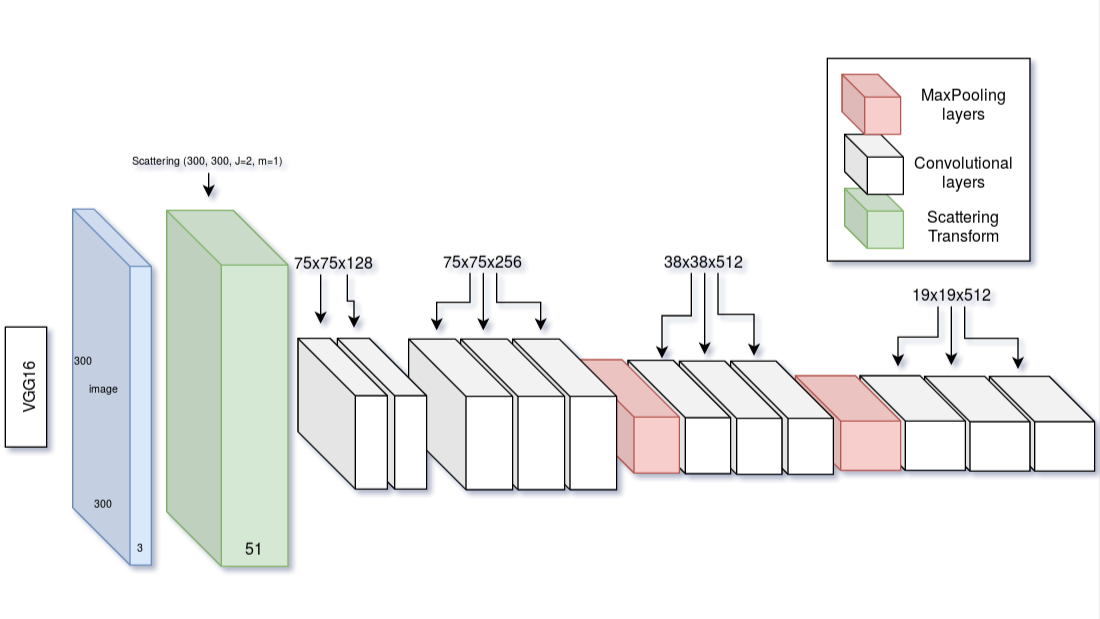
\includegraphics[width=\textwidth]{images/sequential_scattering_ssd.png}}
	\caption{Sequantial scattering SSD. The first two filters are replaced by a scattering transform with $J=2$ and $m=1$. This means the output has $3 \cdot 17 =51$ output channel.}
	\label{fig:sequential_scattering_SSD}
\end{figure}

\subsection{Parallel Scattering}
\label{subsec:parallel_scattering_experiment}

The parallel scattering network was realized by forwarding every image through the conventional pipe and two scattering networks. The first one had $J=m =1$ and the second had $J=m=2$. They were merged with the normal forward pass after the first and second max pooling operation respectively. The number of channels was calculated as described in \ref{eq:order1_num_filters} and \ref{eq:order2_num_filters} and results in 27 and 243 channels for the first and second scattering transformation respectively. A graphical interpretation of the parallel hybrid network can be seen in figure \ref{fig:parallel_scattering_SSD}.  \\
The experiments consisted of training a parallel scattering networks on all available datasets, i.e. Kitti, PASCAL VOC, Toy data, scale toy data, rotation toy data, deformation toy data and translation toy data with the hyperparametrization given by the baseline experiments. Additionally, \textit{pretrained} was tested for all combinations. The results of \textit{pretrained} might contain interesting information about the way in which the scattering networks process their data when confronted with another representation of it. The \textit{batchnorm} makes all results of the parallel scattering very bad and is therefore turned off for the experiments. 

\begin{figure}[!htb]
	\centering
	\fbox{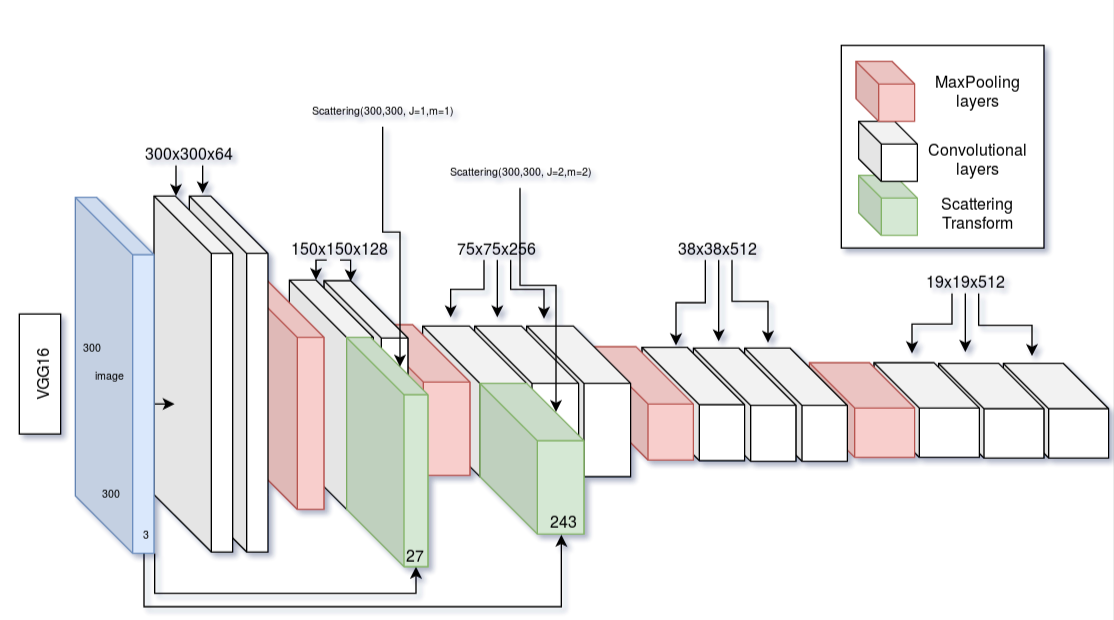
\includegraphics[width=\textwidth]{images/parallel_scattering_vgg.png}}
	\caption{Parallel scattering SSD. The image is piped through the normal VGG path and additionally through a scattering transform with $J=1$ and $m=1$ and a second one with $J=2$ and $m=2$. The outputs of the scattering transforms are concatenated with the other pipe as soon as the dimensions are compatible.}
	\label{fig:parallel_scattering_SSD}
\end{figure}

\subsection{Small Data Experiments}
\label{subsec:small_data_experiments}

One of the possible advantages of filters that need no new training is that their models converge faster and that they generalize better from small sample sizes. Therefore an experiment was run for the toy dataset with only 600 samples for training and 200 for testing. The networks only train 25k epochs instead of 100k. The experiment was conducted for the standard SSD, the sequential scattering and the parallel scattering network respectively. Each network was trained multiple times to prevent outliers from determining the results too much. To test the convergence behavior on small datasets even further a second experiment with only 5k epochs was run for all three network types. To compare the results in a more realistic setting all three network types are also trained on the PASCAL VOC dataset with 25k and 5k epochs respectively. 


\subsection{Timing exeriments}
\label{subsec:timing_experiments}

Especially in object detection online usage of the network is an important goal. In the context of self driving cars, for example, a network that is not able to process data within a given period of time makes the network completely useless since the car is unable to drive efficiently. The experiment will measure the average time of $n=100$ forward passes for the SSD, sequential and parallel scattering on a given dataset. For this experiment every timing run will be on one GPU only since this is the most likely use case for applications. The experiment is conducted on a GeForce GTX 1080 Ti.
